\chapter{Implementazione}
\label{chap:chap4}
Questo capitolo tratta in modo approfondito i dettagli implementativi
che hanno caratterizzato lo sviluppo di \textit{Model Predictive Control}, come 
la scelta dei circuiti di Formula 1 che sono stati utilizzati per testare il sistema e per 
effettuare successivamente le analisi, il risolutore utilizzato, la realizzazione del problema di 
ottimizzazione attraverso il linguaggio \textit{Python}, la fase di \textit{tuning} e altri aspetti tecnici.

\section{Circuiti}
Per mettere alla prova l'algoritmo di \textit{Model Predictive Control} 
sono stati scelti due circuiti di Formula 1 in scala 1:10, ovvero \textit{Spa-Francorchamps} e \textit{Monza}. 
In realtà, prima di far correre il veicolo autonomo su un classico 
circuito, lo si è testato su una mappa rettangolare più semplice, 
corrispondente a una versione modificata di
\textit{``Levine Hallway 2nd Floor''}, la sede del Dipartimento di 
Informatica della \textit{University of Pennsylvania}, la cui versione originale viene fornita
di default all'interno del simulatore.
I circuiti usati per questa tesi sono visibili nella Fig.~\ref{fig:fig11} 
e sono stati scaricati dal GitHub di \textit{F1TENTH}~\cite{f1tenthtracks}, in quanto offre 
diverse mappe di circuiti di F1 in scala 1:10 che possono essere utilizzati all'interno del simulatore.

\begin{figure}[H]
    %\centering
    
\includegraphics[width=.47\textwidth, angle=90]{images/Spa_map.png}\hspace{0.2cm}
    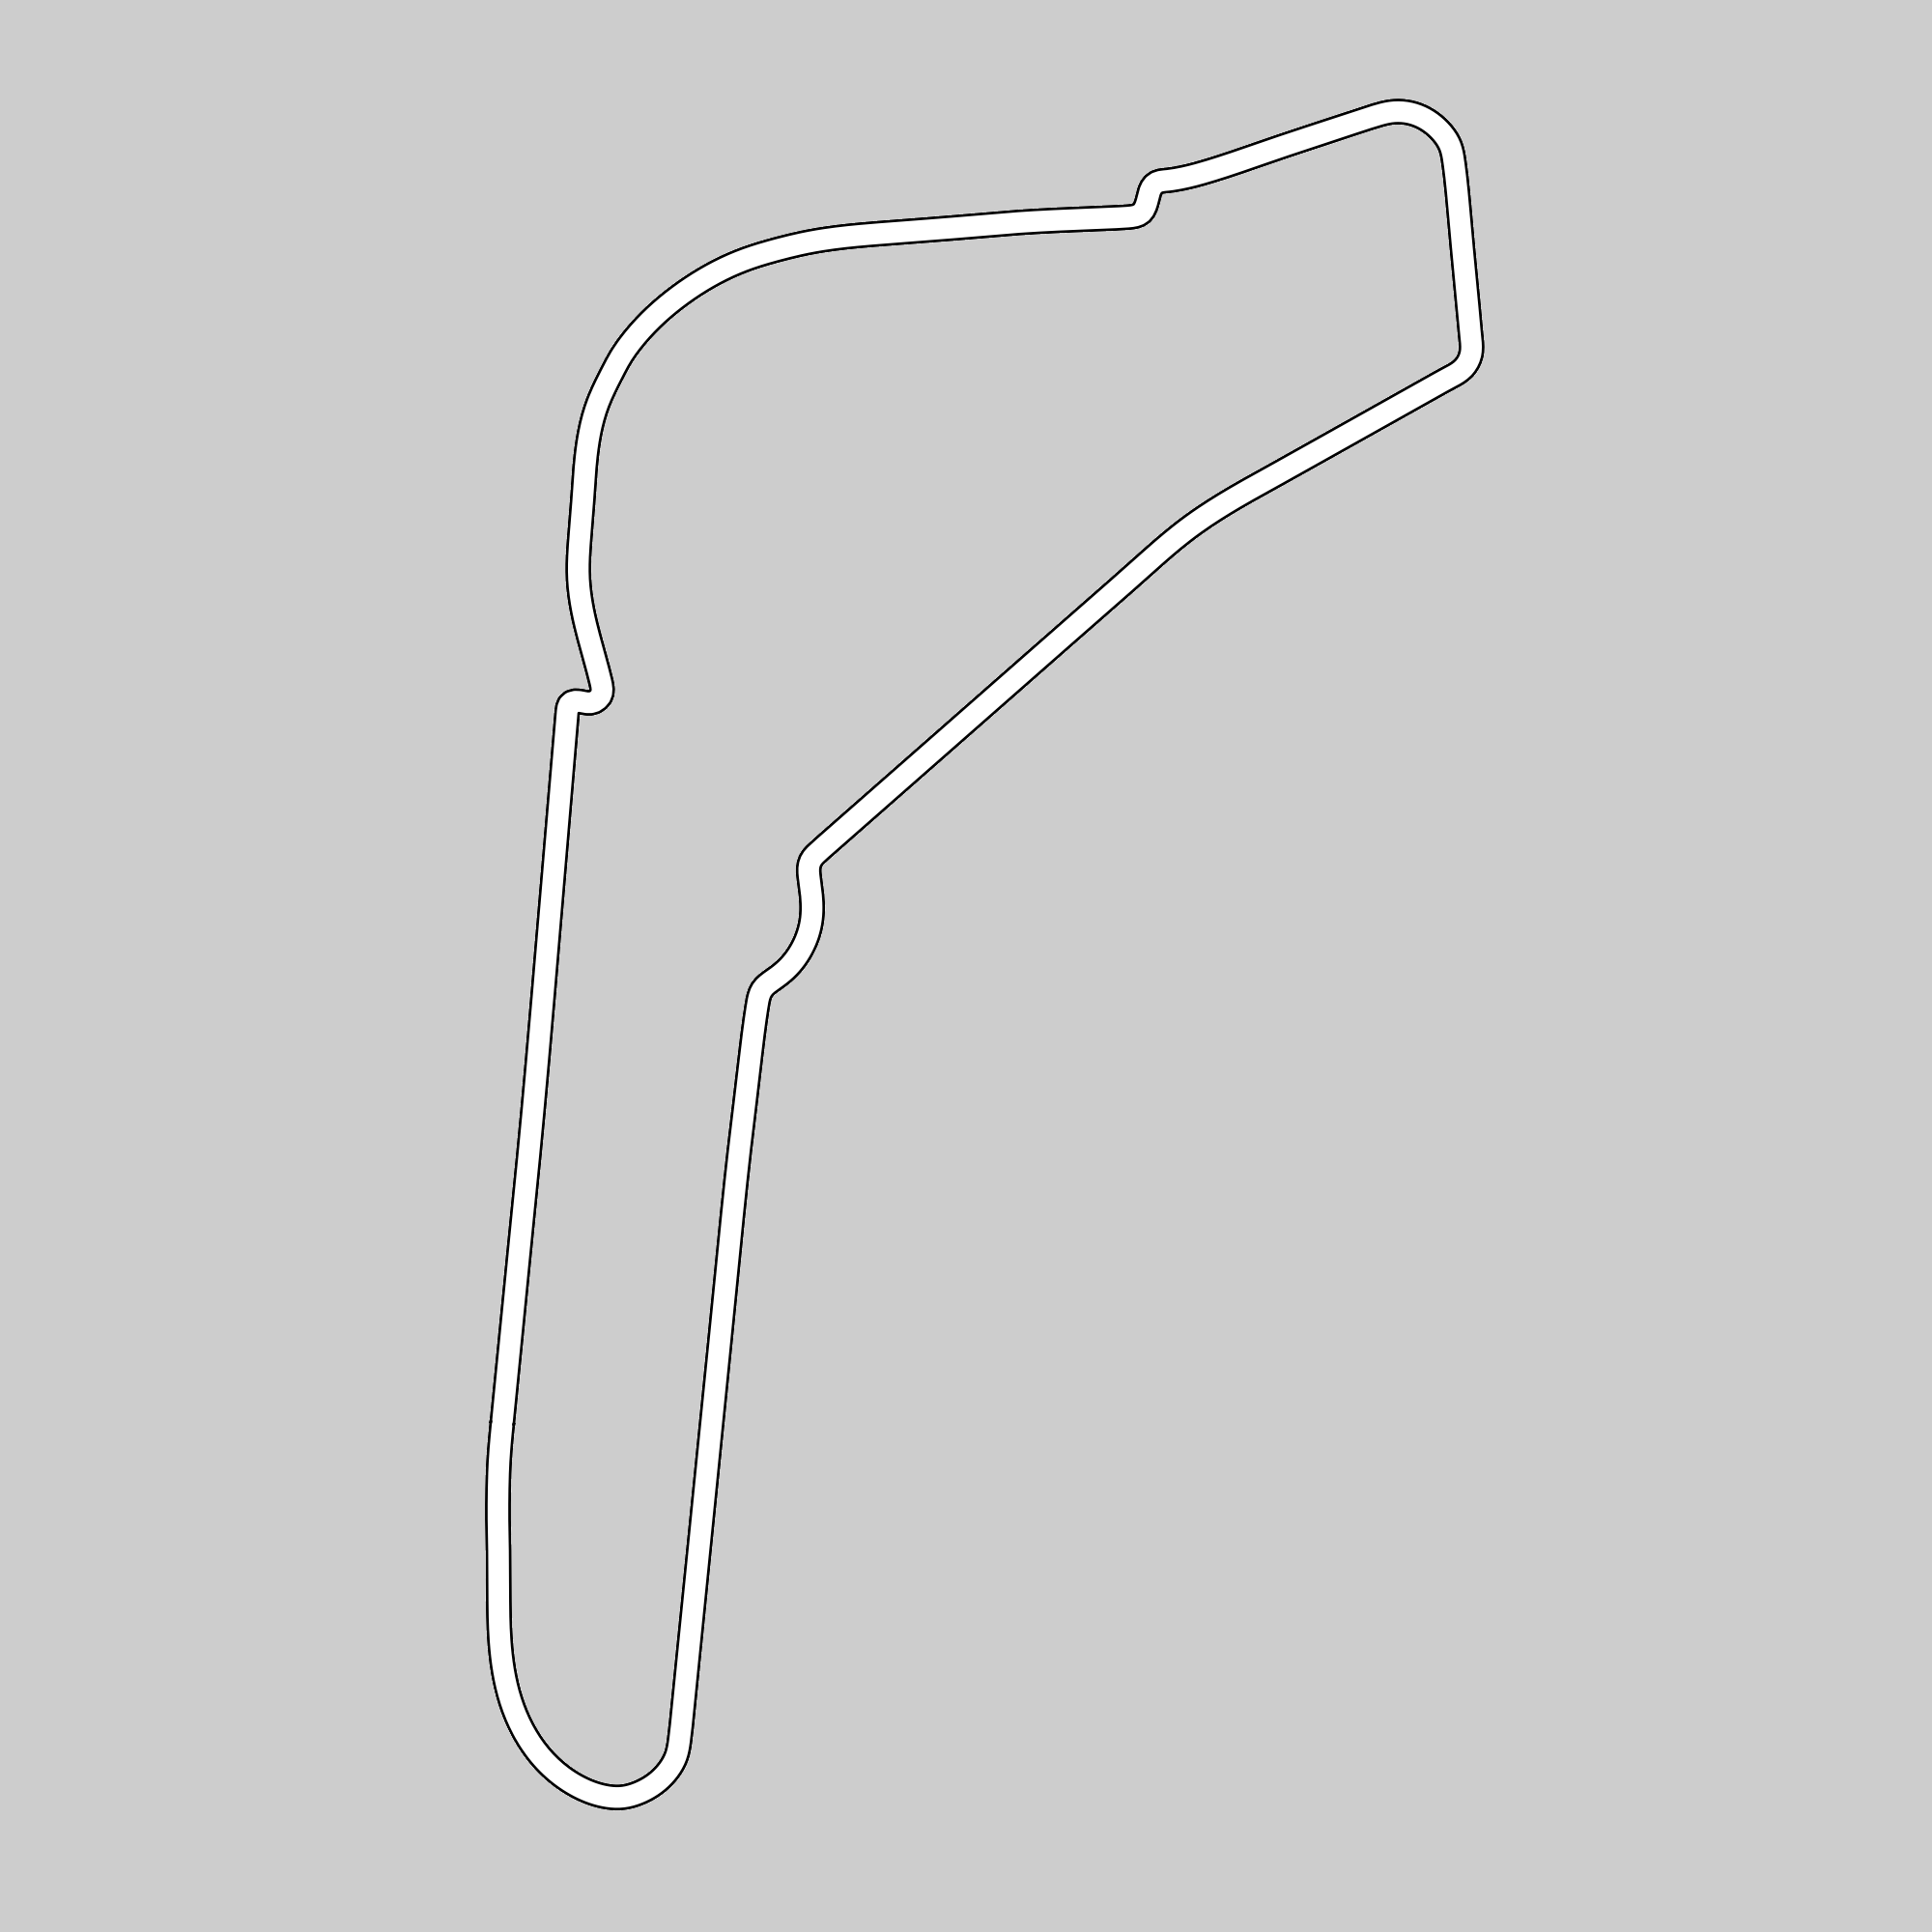
\includegraphics[width=.47\textwidth, angle=90]{images/Monza_map.png}
    \caption{Mappe usate per testare \textit{MPC}~\cite{f1tenthtracks}.}
    \label{fig:fig11} % etichetta utilizzata per riferisi all'immagine
\end{figure}
Ognuna di queste mappe ha comportato un intenso lavoro di adattamento delle 
funzionalità e, in particolare, dei valori di costanti e pesi che 
caratterizzano il \textit{Model Predictive Control}. Questa parte dello 
sviluppo verrà trattata dal punto di vista pratico e implementativo nella 
sezione~\ref{subs:tuning}.

\section{Configurazione}
Prima di poter risolvere il problema di \textit{Model Predictive Control}, è stato necessario 
organizzare i parametri di configurazione che lo definiscono. Essi sono stati riuniti in 
un'apposita classe, utilizzata per definire le caratteristiche ben definite del modello, 
le proprietà fisiche del veicolo, i pesi delle matrici di costo e altri valori necessari per l'ottimizzazione. 
Nello specifico, questi parametri comprendono:
\begin{enumerate}
    \item Dimensioni del modello.
    \begin{itemize}
        \item \verb|NXK|: Dimensione del vettore di stato del veicolo. 
        Gli stati includono posizione \verb|x|, \verb|y|, velocità \verb|v| e orientamento $\theta$.
        \item \verb|NU|: Dimensione del vettore di input di controllo. Gli input includono solo la sterzata $\delta$, interpretata anche come velocità, e l'accelerazione \verb|a|.
        \item \verb|TK|: Orizzonte temporale finito per la previsione dell'algoritmo.
        \item \verb|DTK|: Passo temporale per la previsione, espresso in secondi.
        \item \verb|dlk|: Passo di distanza per la previsione, sempre di 0.03 metri.
    \end{itemize}
    \item Matrici di penalità, anticipate nel Capitolo~\ref{chap:chap3}. I valori utilizzati per queste matrici saranno approfonditi nella sezione~\ref{subs:tuning}.
    \begin{itemize}
        \item \texttt{Rk}: Matrice di costo per gli input di controllo. 
        Penalizza l'uso degli input di controllo, come l'accelerazione e la velocità di sterzata.
        \item \texttt{Rdk}: Matrice di costo per la differenza degli input 
        di controllo. Penalizza i cambiamenti negli input di controllo tra i passi temporali.
        \item \texttt{Qk}: Matrice di costo per l'errore di stato. 
        Penalizza la deviazione dello stato del veicolo -- in ordine
        \verb|x|, \verb|y|, \verb|v| e $\theta$ -- dalla traiettoria di riferimento.
        \item \texttt{Qfk}: Come \texttt{Qk}, ma per lo stato finale del veicolo.
    \end{itemize}
    \item Caratteristiche del veicolo in simulazione.
    \begin{itemize}
        \item \texttt{LENGTH}: Lunghezza del veicolo, di 0.58 metri.
        \item \texttt{WIDTH}: Larghezza del veicolo, di 0.31 metri.
        \item \texttt{WB}: Passo del veicolo, di 0.33 metri.
        \item \texttt{MIN\_STEER}: Angolo di sterzata minimo, che vale -0.4189 radianti.
        \item \texttt{MAX\_STEER}: Angolo di sterzata massimo, che vale 0.4189 radianti.
        \item \texttt{MAX\_DSTEER}: Velocità massima di sterzata, in radianti/secondo.
        \item \texttt{MAX\_SPEED}: Velocità massima del veicolo, di 15 m/s.
        \item \texttt{MIN\_SPEED}: Velocità minima del veicolo, di 0 m/s (per la fase di avvio).
        \item \texttt{MAX\_ACCEL}: Accelerazione massima del veicolo, generalmente di
        3 m/s$^2$.
    \end{itemize}
\end{enumerate}
Questa configurazione viene utilizzata per inizializzare e per risolvere il problema di 
ottimizzazione di \textit{MPC}. I parametri definiti influenzano direttamente il comportamento
del veicolo in simulazione, il modo in cui viene seguita la traiettoria di riferimento
e la risposta del sistema agli input di controllo.

\section{Risolutore}
Una volta completata la fase di configurazione, si può definire e impostare il problema di 
ottimizzazione. Ciò è stato effettuato attraverso l'utilizzo di \verb|CVXPY|, selezionando \verb|OSQP| come risolutore. 

\verb|CVXPY| è un linguaggio di modellazione open-source per problemi di
\textit{ottimizzazione convessa} che viene distribuito come pacchetto di \textit{Python}.
Esso consente di esprimere un certo problema in un modo naturale che segue la matematica, 
piuttosto che nella forma standard restrittiva tipicamente richiesta dai risolutori,
poiché esso trasforma direttamente il problema in tale forma. 
È contraddistinto dai seguenti concetti:
\begin{itemize}
    \item la classe immutabile \verb|Problem| per definire il problema (con obiettivo e vincoli);
    \item la classe \verb|Variable|, che può rappresentare scalari, vettori o matrici;
    \item la classe \verb|Parameter|, che rappresenta espressioni costanti il cui valore potrebbe essere specificato dopo la creazione del problema;
    \item il metodo \verb|solve|, che accetta argomenti facoltativi che consentono di modificare il modo in cui \verb|CVXPY| risolve il problema. Come effetto collaterale, valorizza gli 
    attributi \verb|status| e \verb|value| sull'oggetto relativo al problema.
\end{itemize}
Questi componenti vengono usati per la \textit{creazione} del problema di ottimizzazione 
quadratica -- che verrà risolto a ogni iterazione per determinare gli input di controllo ottimali -- al fine di inizializzare:
\begin{enumerate}
    \item le variabili di stato e controllo, rispettivamente per gli orizzonti \verb|TK+1| e \verb|TK|;
    \item i parametri per lo stato iniziale e per la traiettoria di riferimento da seguire, con quest'ultimo per l'orizzonte \verb|TK+1|;
    \item le matrici di costo a blocchi diagonali, ripetute per ogni passo temporale \verb|TK|. 
\end{enumerate}
% Ricordare: https://www.cvxpy.org/tutorial/functions/index.html#vector-matrix-functions

\section{Obiettivi}
\label{subs:impl_obj}
La prima implementazione cruciale è stata la formulazione e la creazione del problema
di controllo ottimale con orizzonte finito. Dunque, è stata definita la \textit{funzione obiettivo}, 
suddivisa in tre parti distinte, poi sommate tra loro. I dettagli teorici di queste parti sono 
stati trattati ampiamente nella sezione~\ref{subs:obj}; invece, di seguito si riportano delle porzioni di codice per ognuna di esse.

\paragraph{Dettagli implementativi}
\begin{itemize}
    \item \verb|cvxpy.quad_form|: calcola la forma quadratica di un vettore o di una matrice;
    \item \verb|cvxpy.vec|: converte una matrice in un vettore colonna, concatenando le colonne della matrice;
    \item \verb|cvxpy.diff|: calcola la differenza tra le colonne consecutive di una matrice, 
    quindi, in questo caso, viene fatta tra input di controllo in passi temporali consecutivi.
\end{itemize}
\paragraph{Parte 1} La prima parte dell'obiettivo richiede di gestire 
l'influenza degli input di controllo $u$, da moltiplicare dunque con la matrice di penalità $R$.
%Se NU = 2 e TK = 5, e self.config.Rk è: \[ \mathbf{R}\_k = \begin{bmatrix} 0.001 & 0 \\ 0 & 90.0 \end{bmatrix} \]
%Allora R\_block sarà: \[ \mathbf{R}\_{\text{block}} = \begin{bmatrix} \mathbf{R}_k & 0 & 0 & 0 & 0 \\ 0 & \mathbf{R}_k & 0 & 0 & 0 \\ 0 & 0 & \mathbf{R}_k & 0 & 0 \\ 0 & 0 & 0 & \mathbf{R}_k & 0 \\ 0 & 0 & 0 & 0 & \mathbf{R}_k \end{bmatrix} \] La dimensione di R\_block sarà (10, 10).
\begin{lstlisting}[language=PythonPlus]
# Inizializza R come matrice di costo a blocco diagonale
# R = [R, R, ..., R] (NU*T, NU*T)
R_bl = block_diag(tuple([self.config.Rk] * self.config.TK))
obj += quad_form(vec(self.uk), R_bl)
\end{lstlisting}
La funzione \verb|cvxpy.quad_form| calcola la forma quadratica ($u_k^T R u_k$) per ogni $k$ e somma i risultati per tutti i passi temporali $T$, indicati anche come $N$.
Questa operazione corrisponde alla seguente formula matematica: 
\[
\text{obj}_1 = \sum_{k=0}^{N-1}{u_k^T R u_k}
\]
\paragraph{Parte 2} La seconda parte richiede di gestire 
la deviazione del veicolo dalla traiettoria di riferimento, pesata dalla 
matrice di penalità $Q$, includendo il passo temporale finale, che viene pesato però 
da $Q_N$ (cioè $Q_f$). L'obiettivo viene espresso come: 
\[
\text{obj}_2 = (x_N - x_{ref}^N)^T Q_N (x_N - x_{ref}^N) + \sum_{k=0}^{N-1}{(x_k - x_{ref}^k)^T Q_k (x_k - x_{ref}^k)}
\]
\begin{lstlisting}[language=PythonPlus]
# Inizializza Q come matrice di costo a blocco diagonale
# Q = [Q, Q, ..., Qf] (NX*T, NX*T)
Q_bl = [self.config.Qk] * (self.config.TK)
Q_bl.append(self.config.Qfk)
Q_bl = block_diag(tuple(Q_bl))
obj += quad_form(vec(self.xk - self.ref_traj_k), Q_bl)
\end{lstlisting}
\paragraph{Parte 3} La terza parte richiede di gestire 
la differenza tra un input di controllo e il successivo, pesata dalla 
matrice di penalità $R_d$. L'obiettivo in forma quadratica risultante è:
\[
\text{obj}_3 = \sum_{k=0}^{N-2}{(u_{k+1}-u_{k})^T R_d (u_{k+1}-u_{k})}
\]
\begin{lstlisting}[language=PythonPlus]
# Inizializza Rd come matrice di costo a blocco diagonale
# Rd = [Rd, ..., Rd] (NU*(T-1), NU*(T-1))
Rd_bl = block_diag(tuple([self.config.Rdk] * (self.config.TK-1)))
obj  += quad_form( vec(diff(self.uk, axis=1)), Rd_bl )
\end{lstlisting}
Questa parte dell'obiettivo dunque calcola la forma quadratica delle differenze negli input di 
controllo, penalizzando così grandi cambiamenti negli input di controllo.

\section{Vincoli}
Una volta scritto l'obiettivo, sono stati definiti i \textit{vincoli} di \textit{MPC}.
La parte di preparazione delle matrici del modello della dinamica 
(\verb|A|, \verb|B| e \verb|C|) è stata già data dalla comunità di F1TENTH: le matrici in 
questione descrivono l'evoluzione dello stato del veicolo nel tempo in base agli input di 
controllo; inoltre, vengono convertite in parametri di \verb|CVXPY|, al fine di poter essere 
utilizzate nei vincoli della dinamica del veicolo.
Infatti, a questa fase è seguita l'implementazione effettiva dei vincoli, i quali si possono suddividere in tre parti principali: 
\paragraph{Vincoli dinamici} Questi vincoli rappresentano la dinamica del veicolo. La formula corrisponde a: 
\[
x_{k+1} = A_k x_k + B_k u_k + C_k 
\]
\begin{lstlisting}[language=PythonPlus]
flatten_prev_xk = vec(self.xk[:, :-1])
flatten_next_xk = vec(self.xk[:, 1:])
c1 = flatten_next_xk == \
     self.Ak_ @ flatten_prev_xk + \
     self.Bk_ @ vec(self.uk) + \
     self.Ck_
constraints.append(c1)
\end{lstlisting}
\paragraph{Vincolo sulla sterzata} Questo vincolo limita la variazione della velocità di sterzata 
per evitare cambiamenti troppo rapidi. La formula corrisponde a:
\[
-\delta_\text{max} \leq \delta_{k+1} - \delta_k \leq \delta_\text{max}
\]
\begin{lstlisting}[language=PythonPlus]
dsteering = cvxpy.diff(self.uk[1, :])
c2_lower = -self.config.MAX_DSTEER * self.config.DTK <= dsteering
c2_upper = dsteering <= self.config.MAX_DSTEER * self.config.DTK
constraints.append(c2_lower)
constraints.append(c2_upper)
\end{lstlisting}
\paragraph{Vincoli su stati e input} Questi vincoli impongono limiti sugli stati e sugli input
del veicolo. È compreso anche quello sullo stato iniziale, la cui formula corrisponde a: $x_0 = x_{0k}$.
\newpage
\begin{lstlisting}[language=PythonPlus]
# Stato iniziale
c3 = self.xk[:, 0] == self.x0k
constraints.append(c3)
# Stato
speed = self.xk[2, :]
c4_lower = self.config.MIN_SPEED <= speed
c4_upper = speed <= self.config.MAX_SPEED
constraints.append(c4_lower)
constraints.append(c4_upper)
# Input di controllo
steering = self.uk[1, :]
c5_lower = self.config.MIN_STEER <= steering
c5_upper = steering <= self.config.MAX_STEER
constraints.append(c5_lower)
constraints.append(c5_upper)
acc = self.uk[0, :]
c6 = acc <= self.config.MAX_ACCEL
constraints.append(c6)
\end{lstlisting}

\section{Tuning con le penalità}
\label{subs:tuning}
Il \textit{tuning} delle matrici di penalità è un passaggio cruciale per 
ottimizzare le prestazioni di \textit{MPC}; infatti, le matrici influenzano 
direttamente il comportamento del veicolo, poiché bilanciano il \textit{trade-off} tra la 
minimizzazione dell'\textit{errore di stato} e la limitazione dell'effetto degli \textit{input di controllo}.
La scelta dei pesi è stata effettuata in simulazione mediante un processo 
iterativo di test empirici. Ciò è stato fatto al fine di valutare come le variazioni nei
pesi influenzassero le prestazioni del veicolo, così da trovare anche i valori più critici
per regolare di conseguenza. Come anticipato, i pesi sono stati scelti per mantenere un
equilibrio tra la reattività del veicolo e la stabilità del controllo. 
A partire dai pesi determinati in questa fase, si costruiscono le matrici diagonali a blocchi 
\verb|R_block|, \verb|Rd_block| e \verb|Q_block|, descritte nella sezione~\ref{subs:impl_obj}.

Per la configurazione e la gestione del nodo \textit{ROS} di \textit{MPC} sono stati usati dei 
\textit{launch file}, ciascuno per ogni profilo di guida determinato per quest'algoritmo.
Ogni profilo di guida, detto anche configurazione, è configurato con parametri specifici
per adattarsi alle diverse esigenze operative. Essi consistono in:
\begin{itemize}
    \item \verb|Safe| -- Rappresenta un profilo adatto per una guida 
    più sicura e stabile, in quanto parte a velocità basse per poi salire
    con accelerazione elevata. Considerando un orizzonte temporale non molto alto, applica 
    penalità elevate sull'errore di stato per garantire che il veicolo segua accuratamente la traiettoria di riferimento.
    \item \verb|Fast| -- Questo profilo è bilanciato tra velocità e stabilità, con valori
    di velocità massima di sterzata inferiore. Inoltre, a seconda del circuito, ha penalità
    sugli input di controllo leggermente superiori rispetto al profilo \verb|Safe|, in modo da 
    favorire una risposta più rapida del sistema.
    \item \verb|High Performance| -- Si tratta di un profilo configurato per una guida
    estremamente reattiva e rapida. Esso presenta un orizzonte temporale più ampio e penalità 
    generalmente inferiori sull'errore di stato e sugli input. Ciò permette al veicolo di 
    rispondere rapidamente ai cambiamenti nella traiettoria.
\end{itemize}

%\subsection{Levine}
\subsection{Spa}
Nella Tabella~\ref{tab:spa_mpc_profiles} sono indicati i valori scelti per ciascuna configurazione 
relativa al circuito di \textit{Spa}. I valori presenti riguardano i parametri del modello, quelli del veicolo e i pesi delle matrici di penalità.

\begin{table}[H]
\centering
\begin{tabular}{|l|c|c|c|}
\hline
\textbf{Parametro} & \textbf{Safe} & \textbf{Fast} & \textbf{High Performance} \\
\hline
\verb|TK| & 5 & 5 & 7 \\
\verb|DTK| & 0.03 s & 0.03 s & 0.03 s \\
\verb|MAX_SPEED| & 15 m/s & 15 m/s & 15 m/s \\
\verb|MAX_ACCEL| & 10 m/s$^2$ & 3 m/s$^2$ & 3 m/s$^2$ \\
\verb|MAX_DSTEER| & 180°/s & 90°/s & 45°/s \\
\verb|Rk| & [0.001, 90] & [0.001, 90] & [0.001, 110] \\
\verb|Rdk| & [0.1, 500] & [0.1, 600] & [0.001, 110] \\
\verb|Qk| & [60, 60, 30, 60] & [70, 70, 30, 70] & [70, 70, 5.5, 60] \\
\verb|Qfk| & [60, 60, 30, 60] & [70, 70, 30, 70] & [70, 70, 5.5, 60] \\
\hline
\end{tabular}
\caption{Confronto dei profili di MPC per il circuito di Spa.}
\label{tab:spa_mpc_profiles}
\end{table}

\subsection{Monza}
Similmente, per il circuito di \textit{Monza} nella Tabella~\ref{tab:monza_mpc_profiles} sono
riportati i valori scelti per ciascuna configurazione.

\begin{table}[H]
\label{tab:monza}
\centering
\begin{tabular}{|l|c|c|c|}
\hline
\textbf{Parametro} & \textbf{Safe} & \textbf{Fast} & \textbf{High Performance} \\
\hline
\verb|TK| & 5 & 5 & 7 \\
\verb|DTK| & 0.03 s & 0.03 s & 0.03 s \\
\verb|MAX_SPEED| & 15 m/s & 15 m/s & 15 m/s \\
\verb|MAX_ACCEL| & 10 m/s$^2$ & 3 m/s$^2$ & 3 m/s$^2$ \\
\verb|MAX_DSTEER| & 180°/s & 45°/s & 45°/s \\
\verb|Rk| & [0.001, 90] & [0.005, 80] & [0.01, 100] \\
\verb|Rdk| & [0.1, 750] & [0.1, 750] & [0.01, 100] \\
\verb|Qk| & [200, 200, 20, 200] & [200, 200, 20, 200] & [50, 50, 5.5, 50] \\
\verb|Qfk| & [200, 200, 20, 200] & [200, 200, 20, 200] & [50, 50, 5.5, 50] \\
\hline
\end{tabular}
\caption{Confronto dei profili di MPC per il circuito di Monza.}
\label{tab:monza_mpc_profiles}
\end{table}

\section{Visualizzazione}
L'algoritmo \textit{MPC} viene visualizzato su \verb|RViz| attraverso la 
pubblicazione di \verb|Marker| appartenenti a \textit{ROS}, osservabili nella Fig.~\ref{fig:fig12}.
\begin{figure}[H]
    \centering
    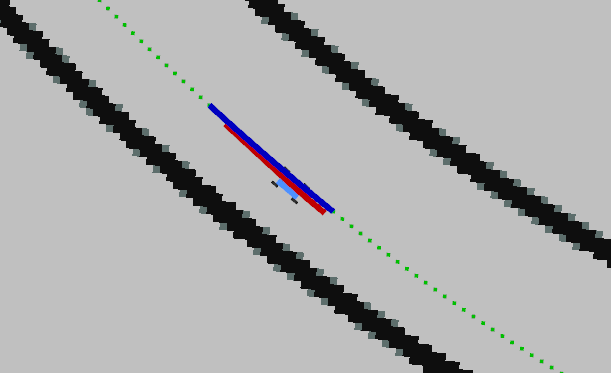
\includegraphics[scale=0.7]{images/mpc_viz.png}
    \caption{Visualizzazione dei ROS topic utilizzati per \textit{MPC}.}
    \label{fig:fig12} % etichetta utilizzata per riferisi all'immagine
\end{figure}
Per visualizzare l'algoritmo si creano e, infine, si pubblicano i marker che rappresentano:
\begin{itemize}
    \item i \textit{waypoints}, che rappresentano i punti di riferimento che il veicolo deve seguire;
    per mostrarli si utilizza un marker verde di tipo \verb|POINTS|.
    \item la \textit{traiettoria di riferimento}, ovvero la traiettoria ideale che il veicolo dovrebbe 
    seguire, mostrata mediante un marker blu di tipo \verb|LINE_STRIP|.
    \item il \textit{percorso predetto}, cioè la traiettoria che il veicolo seguirà in base agli input di 
    controllo attuali, mostrata con un marker rosso di tipo \verb|LINE_STRIP|.
\end{itemize}
Tuttavia, si specifica che per visualizzare i marker pubblicati è necessario aggiungere delle nuove 
schermate di tipologia \verb|Marker| su \verb|RViz|, per ciascuna delle tre visualizzazioni. 
Inoltre, bisogna configurare correttamente i \verb|topic| su cui si pubblicano i marker definiti, ad esempio, per i waypoints è stato scelto il nome ``\verb|/visualization_waypoints|''.